\documentclass[12pt]{article}
\usepackage[left=0.5in, right=0.5in, top=0.75in, bottom=0.5in]{geometry}
\usepackage{epsfig,graphics,amsmath,color,multicol,enumitem,tabularx,pbox,url}
\usepackage{cancel}
%\usepackage[firstpage]{draft watermark}

\setlist{noitemsep}
\setlist{nolistsep}

\pagestyle{empty}

\newenvironment{boxe}
    {\begin{center}
    \begin{tabular}{|p{0.9\textwidth}|}
    \hline\\
    }
    { 
    \\\hline
    \end{tabular} 
    \end{center}
    }

\begin{document}


\begin{tabular*}{\textwidth}{@{\extracolsep{\fill}}l l}
\textbf{Exam 2 Practice}  &  Create a Calculus pun: \hrulefill \\
%\textbf{\today} & MATH 157, Hogwart's House: \rule{4cm}{0.5pt}  \\
\textbf{Math 160 } & \hspace{15cm} \\
\hline\hline
\end{tabular*} 


\normalsize 

\vspace{.4cm}
This work sheet only looks at Standards . The exam also covers 
\begin{enumerate}
    \item(S3) Let $f(x)=\frac{|x-1|}{x}$. Use the limit definition to compute $f'(-1)$
    \vfill
    \item Standard D6(D4+D5): $\displaystyle{w(x)=\frac{2\sin(x)4^x}{x^6}}$. Identify what rules you will need and then find $w'(x)$
    \vfill
    
    \newpage
    \item Standard D2: Use a linearization to approximate $2^{2.8}$ and determine if your approximation is an overestimate or underestimate.
    \vfill
    \item If the graph below is of the {\bf derivative}, $f'(x)$, sketch a possible graph of the parent function, $f(x)$. (Hint: First determine where the parent function $f(x)$ must be increasing/cecreasing CCU/CCD)
    \vspace{4cm}
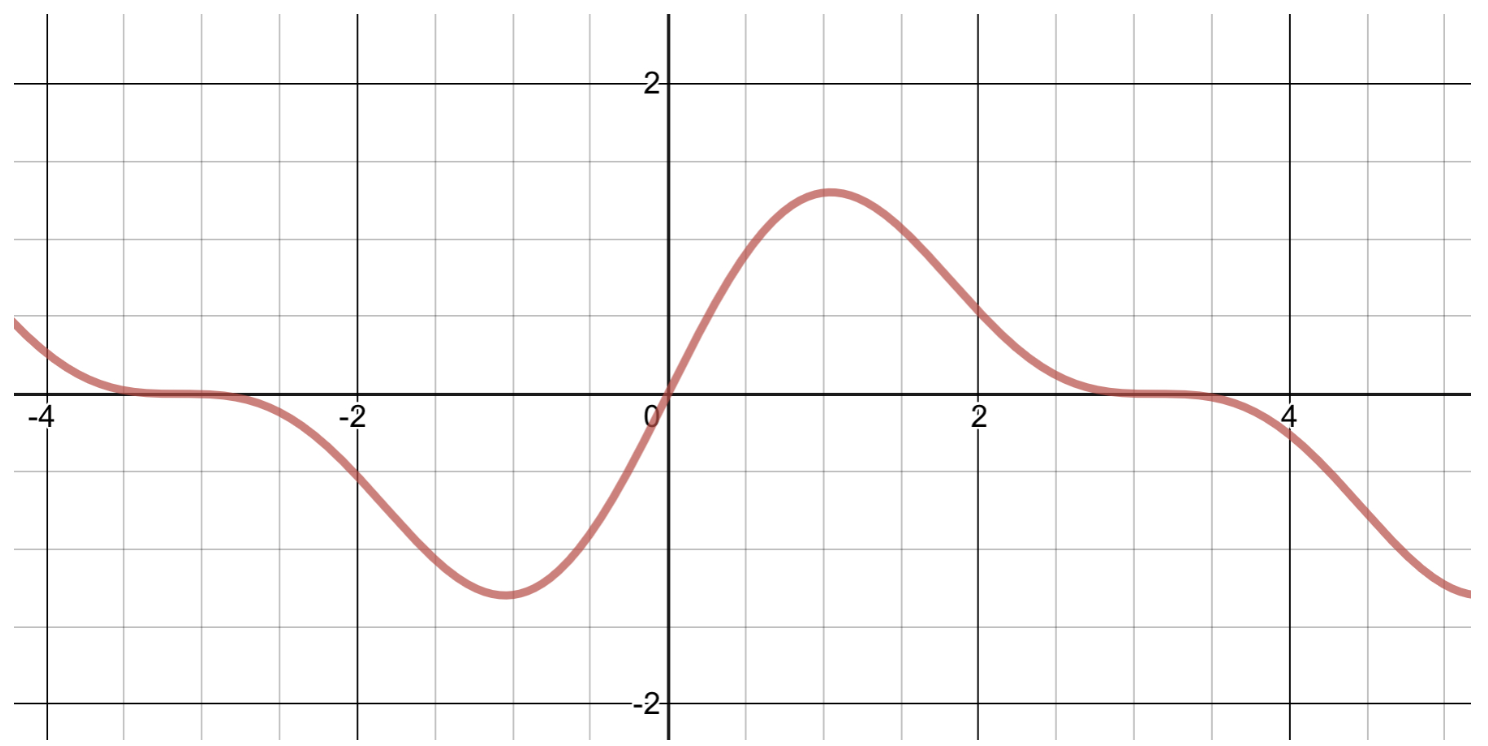
\includegraphics[scale=0.5]{D3graph1.png}
    \item If you have not completed the Exam prep document, do that now!!
\end{enumerate}




\end{document}
